\documentclass[a4paper]{article}
\usepackage[utf8]{inputenc}
\usepackage[english, italian]{babel}
\usepackage{microtype} % tipografia
\usepackage{graphicx}
\usepackage[bookmarks=true,bookmarksopen=true,pdfhighlight=/I,pdfpagemode=UseOutlines]{hyperref} % hyper-links, questo va per ultimo


\makeindex

\begin{document}
\title{Relazione del progetto di \\Sistemi Distribuiti}
\author{Elia Calligaris e Paolo Snidaro}
\date{\textit{bozza} - \today}
\maketitle
\tableofcontents

\section{Introduzione}\label{sec:intro}

Il problema proposto è quello di implementare un protocollo di transazioni distribuite, tramite il quale dei client possono prenotare in modo concorrente delle risorse disposte su più server.

\paragraph{Il pretesto} è quello di gestire un sistema di prenotazione di posti su voli aerei. Idealmente un'agenzia di viaggio (client) deve essere in grado di prenotare via internet una serie di posti su più voli di diverse compagnie. I server delle compagnie aeree mantengono la lista e lo stato dei voli e relativi posti. La prenotazione ha successo se e solo se \textit{tutti} i posti richiesti vengono prenotati. 

Naturalmente si vuole evitare che le richieste di prenotazione interferiscono tra di loro (e soprattutto evitare che lo stesso posto venga prenotato più volte). %Nel caso in cui venga richiesto un posto che risulta occupato, il client potrebbe proporre un posto alternativo all'utente (se possibile).

\paragraph{Una soluzione na\"ive} è quella di creare una transazione per ogni posto da prenotare, abortendo nel caso in cui una fallisca; tuttavia si vuole evitare l'annullamento di prenotazioni già effettuate.

%============================================================================
%============================================================================
%============================================================================

\section{Analisi}\label{sec:analisi}

\subsection{Requisiti funzionali}
\begin{itemize}
	\item Ogni agenzia deve poter richiedere i voli e i posti disponibili alle compagnie.
	\item Ogni agenzia deve essere in grado di prenotare atomicamente una serie di posti su voli potenzialmente diversi. A fronte della lista di posti richiesti, viene richiesta la conferma o meno della prenotazione, eventualmente con delle proposte alternative a posti richiesti ma occupati.
	\item Qualora un'agenzia non riesca ad ottenere uno o più posti richiesti, l'intera prenotazione deve essere annullata.
	\item Qualora un client (agenzia) subisca guasti, la transazione va abortita.
	\item Ci devono essere almeno cinque compagnie aeree.
	\item Ogni server di ogni compagnia aerea mantiene una lista di voli, i quali hanno una serie di posti che possono essere liberi o prenotati.
	\item Un posto in aereo non deve mai venire prenotato più volte.
	\item Una volta confermata una prenotazione per un posto aereo, questa non deve essere più annullata dai server.
	\item L'agenzia deve essere in grado di disdire una prenotazione. Si astrae su eventuali termini per l'annullamento.
\end{itemize}

\subsection{Requisiti non funzionali}

\begin{itemize}
	\item Alta disponibilità, almeno $96\%$ (circa un giorno al mese di downtime).
	\item Tempi di risposta contenuti: se una transazione non viene completata entro $N$ secondi, viene abortita (dal client).
		\item Trasparenza rispetto alla replicazione. Una stessa compagnia può avere più server replica; può esporli tutti su indirizzi separati, oppure metterli sotto un singolo indirizzo e gestirli come più opportuno. Se vengono esposti più indirizzi, sarà il client a contattarne di diversi in caso di problemi.
\end{itemize}
\subsubsection{Fault Tolerance}
\begin{itemize}
	\item I server delle compagnie aeree devono cercare di mascherare i \textit{crash}. Un crash durante una transazione causa un \textit{abort}, uno dopo il \textit{commit} non deve causare perdite.
	\item Omissioni di messaggi da parte dei server vengono visti dal client come un \textit{timeout}. Se sono disponibili indirizzi alternativi, il client può decidere di contattarli in modo trasparente.
	\item Omissioni o crash da parte del client portano la transazione ad essere abortita dai server.
\end{itemize}

%============================================================================
%============================================================================
%============================================================================

\section{Progetto e specifiche}

\subsection{Architettura logica}
% Componenti, funzioni, utenti

L'architettura è di tipo \textit{client-server} a due \textit{tier}, con server \textit{peer} (dato che le risorse sono distribuite).

I \textbf{server} delle compagnie aeree mantengono la lista di voli e di posti a sedere, tendendo conto se quest'ultimi sono occupati o meno (e da chi). Forniscono la lista dei posti su richiesta. Possono eliminare una prenotazione effettuata da un client (su sua richiesta e solo sulle risorse gestite dal server).

I \textbf{client} delle agenzie di viaggio interrogano i server (conosciuti a priori) per avere la lista dei posti, e richiedono la prenotazione di una lista di posti. I client sono operati dagli addetti delle agenzie di viaggi.

Ogni server possiede una lista di aerei, ognuno identificato da un codice; ogni aereo contiene una lista di posti numerati, tenendo traccia del relativo stato (occupato/libero).

%============================================================================

\subsection{Protocolli e algoritmi}
% Comunicazioni tra componenti, UML sequenza, descrizione algo. distrib.
\begin{figure}[t]
	\centering
		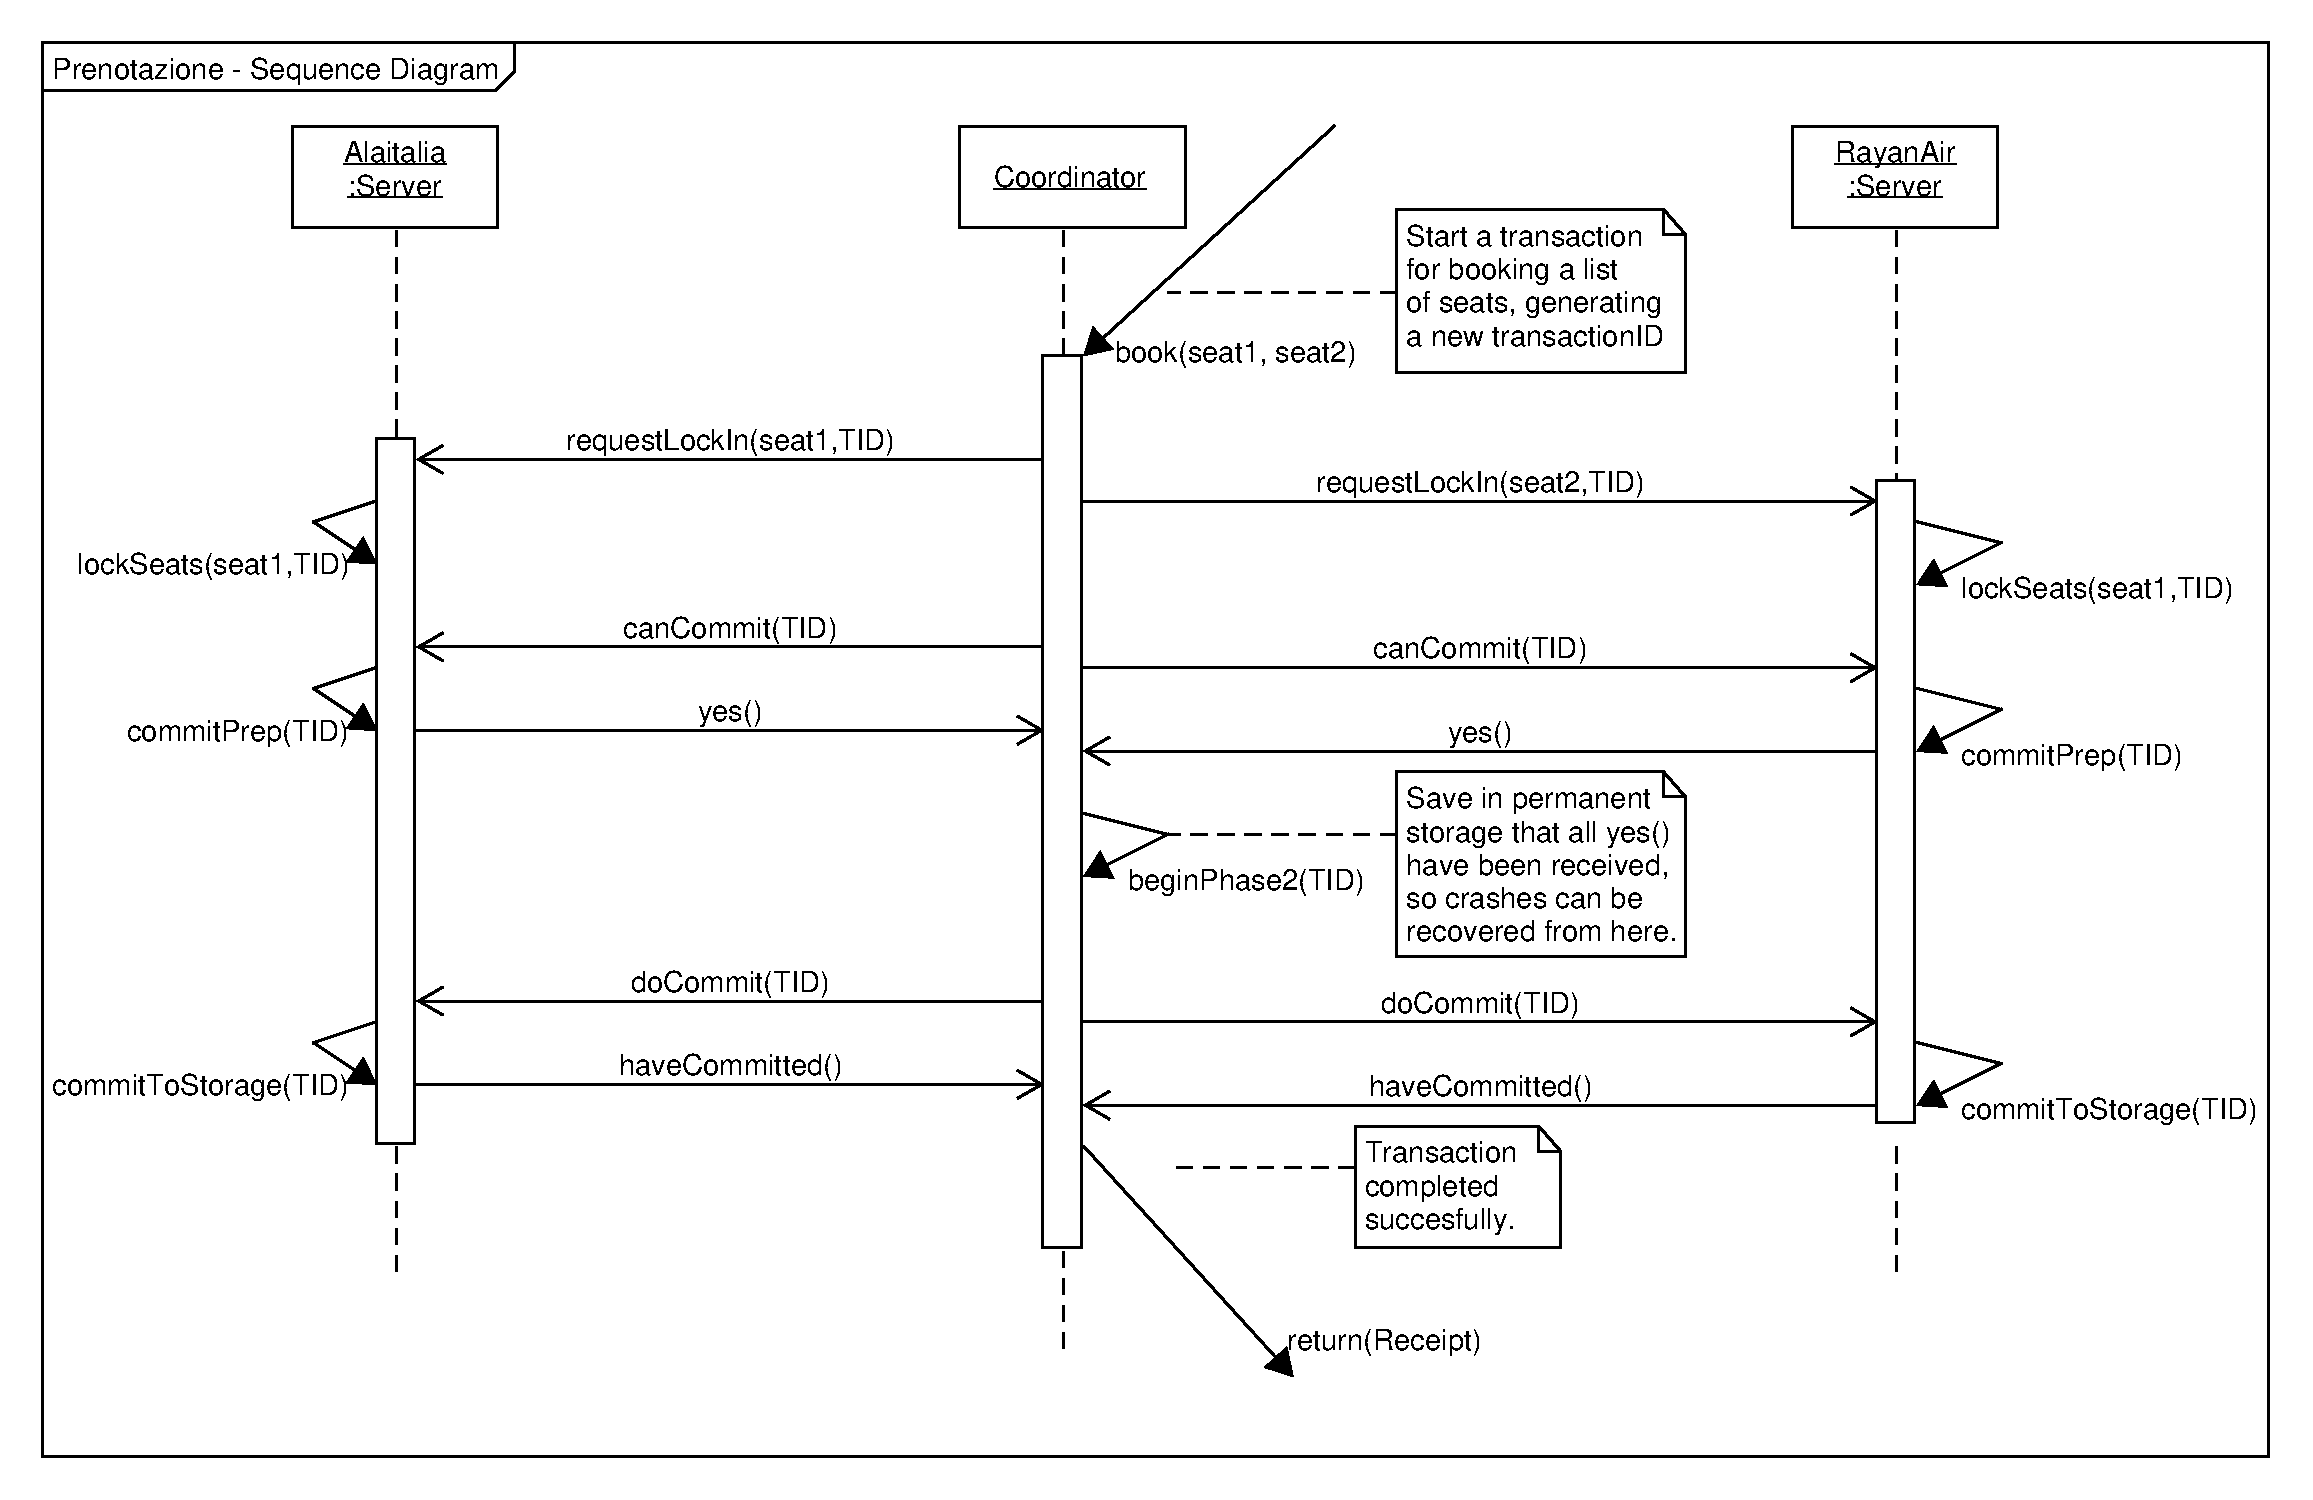
\includegraphics[width=\textwidth]{fig/reserve_sequence.pdf}
		\caption{Diagramma di sequenza UML di un'operazione di prenotazione di due posti, eseguita con successo.}
		\label{fig:bookseq}
\end{figure}

\paragraph{Lista posti}La richiesta della lista di posti disponibili è una semplice interrogazione di tipo \textit{request-reply}: il server invia la lista di tutti i voli e relativi posti, compreso il loro stato (disponibile/occupato).

Ogni aereo è identificato da una sigla (e.g. "AB0123") e ogni posto è identificato da un numero crescente maggiore di zero, unitamente al relativo volo.

\paragraph{Prenotazione}Come mostrato in figura \ref{fig:bookseq}, l'operazione di prenotazione consiste nel richiedere il \textit{lock} delle risorse ai server coinvolti, per poi inizializzare un \textit{two phase commit protocol}.
Se le risorse non sono disponibili, allora il protocollo 2PC farà abortire la transazione.

Tutte le parti coinvolte sfruttano dei file di \textit{log} o dei \textit{database} per eseguire il recupero dai guasti.

Più in dettaglio, la prenotazione consiste delle seguenti fasi:
\begin{itemize}
	\item Uno dei server riceve la richiesta di prenotazione dal client, diventando coordinatore;
	\item Il coordinatore invia ai server coinvolti nella transazione un messaggio \textit{requestLock}, a seguito di cui essi riservano le risorse richieste (se possibile);
	\item Fatto questo, il coordinatore invia un \textit{canCommit} ai partecipanti, a cui ognuno risponde \textit{sì} qualora sia in grado di rendere permanenti le modifiche richieste, facendo inoltre in modo che queste non vadano perse in caso di guasti;
	\item Una volta ricevuto \textit{sì} da tutti, il coordinatore invia \textit{doCommit} ai partecipanti, finalizzando la procedura;
	\item Una volta inviati tutti i messaggi, il coordinatore ritorna una ricevuta al client, che verrà richiesta per modificare o annullare la prenotazione.
\end{itemize}

\paragraph{Guasti e recupero} Qualora almeno un partecipante risponda \textit{no} al \textit{canCommit}, la transazione abortisce. Qualora ci sia qualche guasto (o timeout) prima che tutti i partecipanti rispondano \textit{sì}, la transazione abortisce. Oltre quel punto, i partecipanti si sono impegnati a mantenere le modifiche: dovesse qualcosa andare storto, saranno loro a recuperare le modifiche fatte fino a quel punto, e chiedere al coordinatore qualora abbia deciso di finalizzare la procedura o abortire.

%============================================================================

\subsection{Architettura fisica}
% Nodi e piattaforme coinvolte, dove vengono piazzati
I nodi logici corrispondono a quelli fisici:
\begin{itemize}
	\item Ogni server di ogni compagnia aerea sarà su una macchina apposita connessa a Internet, situata dove più opportuno;
	\item Ogni client girerà sulla macchina dell'agenzia di viaggio, connessa a Internet (quindi anche un semplice PC).
\end{itemize}

%============================================================================
%============================================================================
%============================================================================

\section{Implementazione}
%Details about the implementation: every choice about platforms, languages,
%software/hardware, middlewares, which has not been decided in the require-
%ments.
%Important choices about implementation should be described here; e.g.,
%peculiar data structures.

L'implementazione è stata realizzata con il linguaggio \textit{service-oriented} Jolie. Ciò ha portato a notevoli semplificazioni nell'invio di messaggi e della parallelizzazione: infatti il sistema prevede un gran numero di invii di messaggi e scritture su database. La scelta ha anche portato ad alcune complicazioni nell'implementazione delle routine di recovery, a causa del flusso di esecuzione dei programmi in Jolie.

\subsection{Server}
% Server
%	Operazioni
%	Tabelle DB
%	Tipi e interfacce
Un server deve poter assumere a due ruoli: quello di \textit{coordinatore} di una transazione, o di \textit{partecipante}. Un server può coordinare una transazione che lo coinvolge come partecipante.

\paragraph{Interfacce}I server espongono due interfacce:
\begin{itemize}
	\item \texttt{Coordinator} per le operazioni da coordinatore (apertura transazione, \texttt{getDecision})
	\item \texttt{FlightBookingInterface} per le altre operazioni necessarie alle transazioni, e per le interrogazioni sui posti disponibili
\end{itemize}
Inoltre ci sono due interfacce "private", chiamate \texttt{Spawn} e \texttt{TransRecovery}: la prima viene utilizzata dai server per generare chiamate parallele delle operazioni di \texttt{FlightBookingInterface}, mentre la seconda viene utilizzata per il recupero dai guasti.

\paragraph{Database}Ogni server ha un proprio database, su cui legge e scrive sulle seguenti tabelle:
\begin{itemize}
	\item \texttt{seat}, che contiene i dati sui posti a sedere, ovvero numero, codice aereo, libero/occupato, e hash della ricevuta se prenotato;
	\item \texttt{trans}, usata per tenere traccia delle modifiche effettuate nel corso di una transazione, e qualora tali modifiche siano temporanee (\textit{tentative}) o meno;
	\item \texttt{coordtrans}, usata dal coordinatore per tenere traccia dei partecipanti a ogni transazione, nonché il relativo stato (modifiche richieste, \textit{can commit}, \textit{committed}, \textit{abort});
	\item \texttt{transreg}, usata da ogni server per tenere traccia delle transazioni a cui partecipa, e del relativo coordinatore;
	\item \texttt{counter}, usata per salvare il contatore delle transazioni eseguite
\end{itemize}


\subsubsection{Interrogazione dei server}
Sono previste due possibili interrogazioni ai server:
\begin{itemize}
	\item \texttt{getAvailableSeats} produce una lista dei posti liberi disponibili presso il server;
	\item \texttt{getReservedSeats} produce, a fronte di una ricevuta, i relativi posti prenotati presso il server.
\end{itemize}


%	Booking (coordinatore)
\subsubsection{Prenotazione posti}
L'operazione di prenotazione inizia con la richiesta da parte del client; essa deve contenere:
\begin{itemize}
	\item un array contenente
	\begin{itemize}
		\item l'indirizzo di un server (partecipante);
		\item una lista di posti (numero e volo) da richiedere al server; opzionalmente a ogni posto di può aggiungere la relativa ricevuta di prenotazione per rimuoverli da quest'ultima;
	\end{itemize}
	\item l'indirizzo del client che effettua la richiesta, in modo da poter essere contattato dal coordinatore per escludere guasti durante l'operazione;
	\item opzionalmente un valore in millisecondi per il tempo massimo consentito per l'operazione (timeout).
\end{itemize}

Il server che riceve la richiesta diventa coordinatore della transazione, eseguendo le seguenti operazioni:
\begin{itemize}
	\item genera un nome per la transazione (nome server+contatore transazioni), detto anche \texttt{tid};
	\item fa partire un timer, al termine del quale la transazione viene abortita qualora i partecipanti non siano pronti al \textit{commit};
	\item genera una ricevuta per la transazione (una stringa) e la sua \textit{hash} MD5;
	\item invia a ogni partecipante un messaggio \texttt{requestLockIn} in modo parallelo, tramite l'operazione \texttt{spawnReqLock};
	\item dopo una breve attesa, per dar tempo ai partecipanti di processare il messaggio ricevuto, invia a ogni partecipante un messaggio \texttt{canCommit} in modo parallelo, tramite l'operazione \texttt{spawnCanCommit};
	\item viene inviato \texttt{canCommit} anche al client, per verificare che sia ancora funzionante;
	\item se tutti rispondono \textit{sì} a \texttt{canCommit}, il coordinatore invia ai partecipanti il \texttt{doCommit} (tramite \texttt{spawnDoCommit}) e ritorna al client la ricevuta, terminando la transazione con successo;
	\item se almeno un partecipante (o il client) risponde \textit{no}, allora la transazione viene abortita (tramite \texttt{spawnAbort}, che invia parallelamente \texttt{abort}).
\end{itemize}

Qualora ci sia qualsiasi problema di comunicazione la transazione viene abortita, lanciando \texttt{InterruptedException} al client. 

Si noti che, mentre il timer del coordinatore può essere modificato dal client, ce n'è anche uno per i partecipanti, che viene scelto dai rispettivi proprietari.

%	lock
\paragraph{Lock delle risorse}\texttt{spawnReqLock} invia a ogni partecipante, in modo parallelo, la richiesta di prenotare dei posti, passando inoltre una specie di \textit{session ID} (chiamato \texttt{cid}, o \textit{Coordinator ID}) per identificare i messaggi provenienti dal coordinatore; %(evitando quindi di accettare messaggi provenienti da altre fonti)
assieme al \texttt{cid} viene inviata la hash della ricevuta, in modo che i partecipanti possano capire se una richiesta di annullamento è legittima. %(cioè contiene la ricevuta corretta)
Infine viene registrata in \texttt{coordtrans} l'associazione fra \textit{Transaction ID} (\texttt{tid}), \texttt{cid} e partecipante, in modo che messaggi successivi relativi alla medesima transazione vengano inviati con il \texttt{cid} corretto.

\texttt{requestLockIn} fa sì che il partecipante registri in \texttt{trans} le modifiche richieste; se tutte le risorse sono disponibili viene aggiornata di conseguenza anche \texttt{seat}, altrimenti tutte le richieste di modifica vengono annullate. Viene aggiornata \texttt{transReg} con l'associazione tra \texttt{tid}, coordinatore e \texttt{cid}, facendo sì che tutte le future richieste relative alla transazione \texttt{tid} debbano essere accompagnate da \texttt{cid}.
Inoltre il partecipante fa partire un proprio timer, al termine del quale la transazione viene abortita e le risorse rilasciate.

%	canCommit
\paragraph{Can commit}\texttt{spawnCanCommit} invia a ogni partecipante, in modo parallelo, la richiesta \texttt{canCommit}, ritornando \textit{true} se tutti i partecipanti rispondono \textit{sì}.

\texttt{canCommit} fa sì che il partecipante, a fronte di un \texttt{cid} valido nella richiesta, si impegni a eseguire il \textit{commit} delle modifiche richieste rispondendo con \textit{true}. Nel caso il partecipante non sia in grado di far ciò (a causa di risorse non disponibili o errori), allora risponderà \textit{false}.

%	doCommit
\paragraph{Do commit}\texttt{spawnDoCommit} invia a ogni partecipante, in modo parallelo, la richiesta \texttt{doCommit}, cancellando inoltre il corrispondente record da \texttt{coordtrans}.

\texttt{doCommit} fa sì che il partecipante, a fronte di un \texttt{cid} valido nella richiesta, finalizzi il \textit{commit} della transazione, rimuovendo i relativi record da \texttt{trans} e \texttt{transreg}. % e applicando i cambiamenti a seat

%	abort
\paragraph{Abort}\texttt{spawnAbort} invia a ogni partecipante, in modo parallelo, la richiesta \texttt{abort}, cancellando inoltre il corrispondente record da \texttt{coordtrans}.

\texttt{abort} fa sì che il partecipante, a fronte di un \texttt{cid} valido nella richiesta, annulli tutte le modifiche a \texttt{seat} effettuate durante la transazione, rimuovendo i relativi record da \texttt{trans} e \texttt{transreg}.

%	timeout
\paragraph{Timeout}
Qualora il timeout sia causato dal coordinatore, la transazione viene interrotta e abortita, ma solamente se i partecipanti non hanno ancora risposto positivamente a \texttt{canCommit}.

Se il timeout è causato da un partecipante che non ha ancora risposto \textit{sì} a \texttt{canCommit}, esso abortirà la transazione (e di conseguenza risponderà \textit{no} a un eventuale \texttt{canCommit}).

%	Annullamento
\subsubsection{Annullamento/modifica prenotazione}
Qualora una richiesta di prenotazione posti contenga (come valore opzionale) una ricevuta di prenotazione, questa viene utilizzata per rimuovere suddetto posto da tale prenotazione. Durante \texttt{requestLockIn}, invece di effettuare le relative prenotazioni, vengono rilasciati i posti il cui identificativo e la cui hash della ricevuta corrispondono a quelli inviati con la richiesta.


%	Recovery
\subsubsection{Recupero dai guasti}

Quando un server viene avviato, vengono eseguite tre attività di recupero dai guasti: quella da coordinatore, quella da partecipante e il recupero del contatore delle transazioni. Le attività di recupero sono implementate dal sotto-servizio \textit{embedded} \texttt{transrecovery.ol}.

\paragraph{Recupero da coordinatore} L'attività consiste nel cercare in \texttt{coordtrans} record di transazioni pronte a essere finalizzate, cioè quelle in cui tutti i partecipanti hanno risposto a \texttt{canCommit}. Se il risultato è positivo vengono inviati i \texttt{doCommit}, altrimenti vengono inviati degli \texttt{abort}.

\paragraph{Recupero da partecipante} L'attività consiste nel cercare in \texttt{transreg} record di transazioni aperte. Per ognuna di esse, si leggono i relativi record in \texttt{trans} per verificare qualora ci fosse stato un impegno a eseguire il \textit{commit} o meno: in caso affermativo, vengono fatte delle interrogazioni \texttt{getDecision} al coordinatore (con \textit{backoff esponenziale}), con lo scopo di sapere se finalizzare la transazione o abortire; altrimenti questa viene abortita.

\subsection{Client}
% Client
%	Tabelle DB
%	Tipi e interfacce
Il servizio client invia richieste di prenotazione (o modifica/annullamento) ai server, rimanendo disponibile a rispondere ai loro messaggi di controllo.

\paragraph{Interfacce} Il servizio client espone due interfacce:
\begin{itemize}
	\item \texttt{ClientInterface} che permette ai server coordinatori di verificare se il client è ancora funzionante;
	\item \texttt{InternalClientInterface} che permette all'(ipotetica) applicazione usata dall'utente di iniziare una prenotazione, per cui il servizio client farà da tramite con i server. 
\end{itemize}

Si noti che, in mancanza di un'applicazione per l'utente finale, le prenotazioni possono essere inizializzate tramite un semplice programmino Jolie con \texttt{execution\{single\}}, come ad esempio \texttt{clientStarter.ol}.

\paragraph{Database} Il client mantiene una sola tabella \texttt{receipt}, in cui salva le ricevute delle prenotazioni effettuate.

%============================================================================
%============================================================================
%============================================================================

\section{Validazione}
%Check if requirements from Chapter 2 have been fullled. Quantitative tests
%(simulations) and screenshots of the interfaces are put here.

%============================================================================
%============================================================================
%============================================================================

\section{Conclusioni}
%What has been done with respect to what has been promised in Chapters 1
%and 2, and what is left out.

%============================================================================
%============================================================================
%============================================================================

\appendix
% codice, istruzioni di installazione, ... 

\end{document}














